% Chapter Template

\chapter{Methodology} % Main chapter title

\label{c4} % Change X to a consecutive number; for referencing this chapter elsewhere, use \ref{ChapterX}


 
% \section{Methodology}
This section describes the methodology for tracking accurate temperature prediction using DL techniques on time series data originating from Delhi. The foundation of our study rests on the comprehensive collection and preprocessing of temperature data. We sourced our dataset from reputable weather stations in Delhi from the NASA website, spanning a specific period critical for climate analysis. We conducted rigorous cleaning procedures to ensure data integrity, handle missing values, detect and address outliers, and remove duplicates. Additionally, we performed feature engineering to extract relevant temperature-related features, enhancing the granularity of our Dataset for DL model input.

The exploration of the data's underlying characteristics was undertaken through Exploratory Data Analysis (EDA). Visualization tools, such as line plots and histograms, facilitated the identification of critical temporal patterns and anomalies within the temperature time series. Statistically, we employed various analytical methods during EDA to unveil underlying trends and seasonality.

We selected the LSTM, Bi-LSTM, GRU and RNN DL architecture for the heart of our temperature prediction. Bi-LSTM networks are well-suited for modelling sequential data and capturing long-term dependencies, making them a natural choice for time series forecasting. To optimize model performance, we meticulously tuned hyperparameters, including network depth, hidden unit configurations, activation functions, and dropout rates.



\begin{figure}[ht!]
\centering
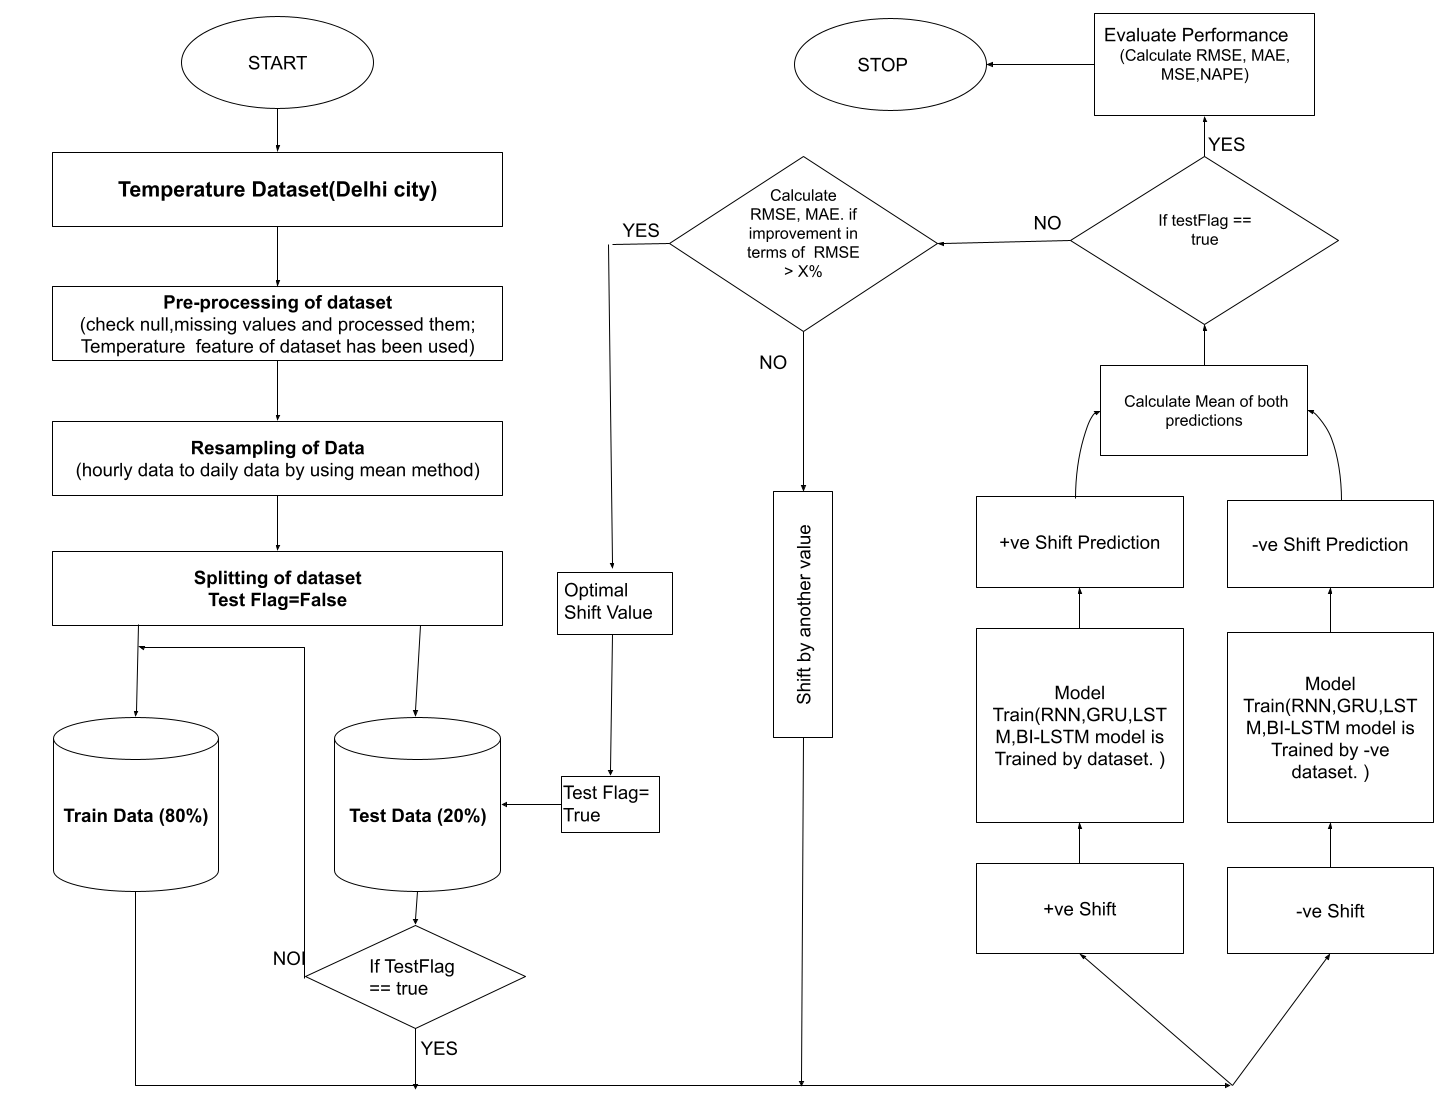
\includegraphics[width=1\textwidth, height=0.9\linewidth]{FlowchartOfjournal.png}
\caption{Framework of the proposed work MBiS-DT + DL models}
\label{fig:Flowchart Of Proposed Work}
\end{figure}
\section{Data collection and preprocessing}
\subsection{Raw dataset collection}
The dataset used in this study is publicly accessible on NASA's website . The dataset contains 195101 rows in CSV format of temperature and dew point of New Delhi from 02/01/2001 to 06/04/2023 on an hourly frequency. The T2M are distinct kinds of atmospheric conditions. These conditions define the atmosphere's temperature for each record in the dataset D, shown in eqn. (\ref{eqn:d}).

\begin{equation}
\label{eqn:d}
D=\left \{ x_i, y_i \right \}_{i=1}^{k}
\end{equation}

where, D is denoted as dataset, \(x_i\) is a temperature data of hours interval, and \(y_i\) its corresponding time. k denotes the number of samples in the dataset, $\forall y_i \in y $.

\subsection{Data preprocessing}
This technique phase consists of four phases. First, dataset D has been resized into a new dimension daily. The function representing the dimension is omega. As shown in eqn.- (\ref{eqn:c}), we also organized the data by date and time and examined the dataset's non-linearity. Furthermore, temperature(T2M) values between 2001 and 2023 have been chosen from the resized dataset. Each date from January 2, 2001, to April 6, 2023, is placed in the dependent variable column, and each item in that column of time series data for 22 years (2001-2023) having temperature (T2M) as an independent variable column has been added.

\begin{equation}
\label{eqn:c}
D_{new}=\omega \left ( D, p \times q \right )
\end{equation}

where, \(D_{new}\) is the preprocessed the dataset D. Here, p x q are the new dimension of the dataset.
\subsection{Exploratory data analysis(EDA)}

% \begin{table*}[h!]
% \caption{statistical summarization of Data set}
% \label{tab: statistical_data_explore }
% \begin{tabular}{ll}
% \hline parameters & Values \\ \hline
% count & 195101 \\
% mean & 25.10 \\
% std & 21.73 \\
% min & -999 \\
% 25\% & 18.70 \\
% 50\% & 26.46 \\
% 75\% & 31.98 \\
% max & 48.79 \\ \hline
% \end{tabular}
% \end{table*}
This section explains statistical details about our Delhi temperature dataset. It provides insights into the dataset's size, central tendency, variability, distribution, and range. These statistics serve as a foundational resource for analyzing and interpreting temperature trends in Delhi, supporting various climate-related studies, weather forecasts, and informed decision-making processes. The \textbf{"count"} value 8,128 indicates the dataset's size, revealing that it bound a substantial number of temperature observations or data points. This size underscores the dataset's richness and the depth of information available for analysis, offering a robust foundation for temperature-related insights. The \textbf{"mean"} temperature of 25.49 degrees serves as the arithmetic average of the dataset. It suggests that, on average, the recorded temperatures in Delhi hover around 25.49 degrees. This central tendency measure offers a crucial reference point, representing the typical temperature value within the dataset. The \textbf{"standard deviation"} (std) of 7.77 quantifies the degree of temperature variation or dispersion in the data. A higher standard deviation indicates more significant variability in the recorded temperatures. In this case, the standard deviation of 7.77 implies that temperature readings in Delhi can exhibit substantial fluctuations around the Mean, signifying the presence of diverse temperature patterns.

The \textbf{"min"} value of 6.95 is the most minor observed temperature in the dataset. However, this value appears unusual and may require further investigation. Some previous Values, like -999, often signify missing data or anomalies that warrant scrutiny to ensure data quality and integrity, so it is handled by taking the Mean of the successor and predecessor value of the time-series dataset. The \textbf{"max"} value of 41.81 denotes the highest temperature recorded in the dataset, offering a glimpse into the upper limit of temperature extremes experienced in Delhi. The \textbf{quartile} values—25\% (first quartile), 50\% (median), and 75\% (third quartile)—offer valuable insights into the distribution of temperatures in Delhi. The first quartile at 18.73 indicates that 25\% of temperature readings fall below this level, while the third quartile at 31.48 signifies that 75\% of the temperatures are below this threshold. The median value of 26.85, also the second quartile, represents the middle point of the dataset when arranged in ascending order. Notably, the median is a robust measure of central tendency unaffected by extreme outliers. These quartile values provide context for understanding the spread and distribution of temperature data in Delhi.



\begin{figure}[ht!]
\centering
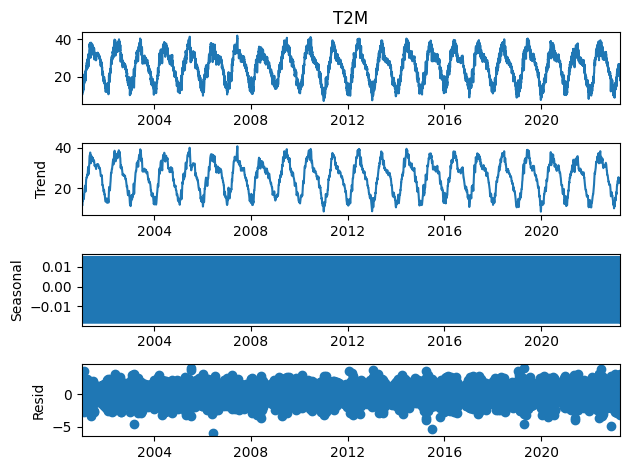
\includegraphics[width=1\textwidth, height=0.75\linewidth]{Graphycal_EDA.png}
\caption{The decomposition of data as a trend, seasonal and residual of Jan. 2001 to Sept. 2001. }
\label{fig:graphycalEDA}
\end{figure}
In our dataset, a good trend is visualized. A trend represents a substantial and meaningful long-term pattern in temperature variations. This pattern provides the fundamental direction in which the 2-meter air temperature changes over an extended period. In climate science, recognizing such trends is vital for understanding the dynamics of temperature variations over time, whether the moderate warming associated with climate change or the multi-year temperature cycles linked to climate phenomena like Delhi. Accurately identifying and modelling these trends is pivotal for climate scientists and meteorologists, as it enables them to make informed projections about future temperature changes, prepare for potential impacts, and implement mitigation strategies.
In the context of our temperature dataset, \textbf{"seasonality"} represents the regular and cyclical fluctuations in temperature that occur at consistent intervals throughout the year. These fluctuations often align with the changing seasons, resulting in patterns like warmer temperatures during summer and colder temperatures during winter. Seasonality in T2M data can be attributed to various factors, including the tilt of the Earth's axis, which leads to variations in sunlight exposure throughout the year. Identifying seasonality in temperature data is critical for climate scientists and ecologists, as it aids in understanding the impact of changing seasons on ecosystems \cite{liu2021modeling}, agriculture \cite{murugesan2021deep}, and human activities. This knowledge is crucial for crop planning\cite{sehgal2017crop}, energy demand forecasting\cite{choi2020power}, and environmental conservation efforts\cite{lee2017using}.

Residuals in our temperature dataset refer to unexplained fluctuations or variations after accounting for the identified trends and seasonality. These residuals represent the difference between the observed 2-meter air temperatures and the values predicted by a model incorporating long-term trends and seasonal patterns. In climate research, analyzing residuals is vital for assessing the accuracy of climate models and identifying any irregular or unanticipated temperature fluctuations. Residuals should exhibit no systematic patterns; if they do, it suggests that the model may need refinement to capture the underlying dynamics of temperature changes better. Effective handling of residuals is essential for producing reliable temperature predictions, which, in turn, inform climate policy\cite{gilik2022air}, weather forecasts\cite{shin2021short}, and resilience planning\cite{ghaith2022synchronization} in the face of temperature-related challenges \cite{lee2020forecasting}.
% \section{Train, and Test Splitting of Dataset}



% \par {\textbf{Step 4}: Applying Deep Learning Models:}\\ the model \(\emptyset\left(D_{Tr}\ ,\ D_{Te}\right)\) has been applied. The forecasting for the test sample has been obtained in the model's training and test part. Prediction is obtained:\(\left\{P_i^\emptyset\right\}_i^m\), where m is number of test sample %\cite{hrithik2022classification}.

% \par {\textbf{Step 5}: Root Mean Squared Error:}\\ RMSE is calculated by eqn. \ref{eqn:e}.



% Where N is total no of test Sample, \(\hat{y_{i}}\) is a predicted data of model, and \(y_{i}\) is the actual test deta.\\
% \par {\textbf{Step 6}: Proposed Technique:} \\
\section{Proposed Multi-Bidirectional Shifting based Data Transformation(MBiS-DT) with DL Model}
\begin{figure}[ht!]
\centering
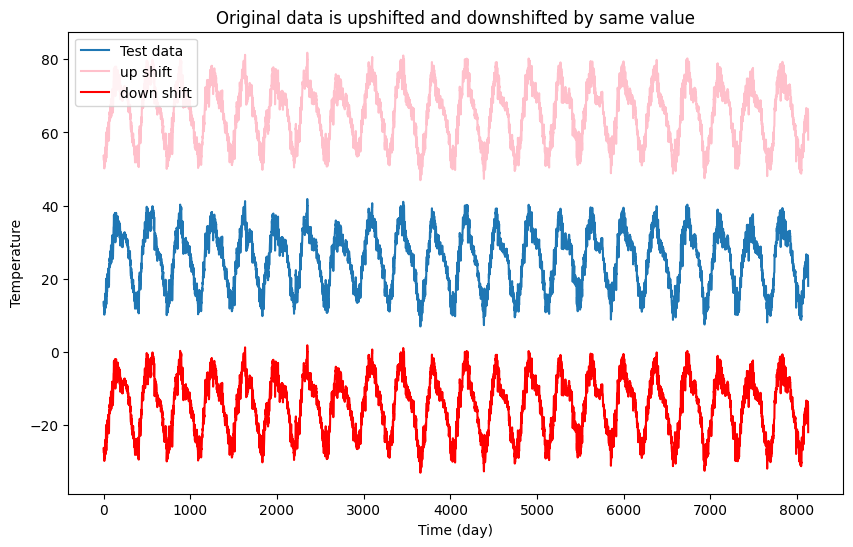
\includegraphics[scale = 0.4]{shifted_dataset.png}
\caption{Pictorial representation of Multi-Bidirectional shifting based Data Transformation(MBiS-DT) for multiple DL learning for the ensemble of models.}
\label{fig:shifted_dataset}
\end{figure}
The preprocessed dataset has been divided into two parts: training \((T_{train})\) (80\%) and testing \((T_{test})\) (20\%). The dataset is mutually exclusive in eqn. (\ref{eqn:a}) and exhaustive in eqn. (\ref{eqn:b}).

\begin{equation}
\label{eqn:a}
D_{T}=D_{Tr}\cup D_{Te}
\end{equation}

\begin{equation}
\label{eqn:b}
\left \{ D_{Tr} \cap D_{Te} \right \}=\varnothing
\end{equation}

For the data points $x_i$ in the training dataset $D_{Tr}$, two series can be created as in eqn. (\ref{eqn:01}):
\begin{equation}
\begin{aligned}
\label{eqn:01}
\{x_i^{\prime}=x_i+s\}_{i=1}^n \\
\{x_i^{\prime\prime}=x_i-s\}_{i=1}^n \; \forall x_i \in D_{Tr}
\end{aligned}
\end{equation}
where $s \in Z$ and $x_i^{\prime}$ and $x_{i}^{\prime\prime}$ depicts the positive and negative series obtained by shifting the series with positive and negative values of the step length $s$ of the shift. The series has been prepared for $n$ number of iterations.
Predictions for both the positive $x_i^{\prime}$ and negative $x_i^{\prime\prime}$ series has been obtained as $\hat{y}_i^{\prime}$ and $ \hat{y}_i^{\prime\prime}$ respectively.
The predictions are combined to form a final set of predictions using eqn. (\ref{eqn:02}), which is utilized to compare with the actual values of training dataset $D_{Tr}$.
\begin{equation}
\label{eqn:02}
\hat{y}_{final}=\frac{y_i^{\prime}+y_i^{\prime\prime}}{2}
\end{equation}
where $\hat{y}_{final}$ represents the final prediction. The above procedure is repeated for $n$-number of iterations, and an optimal value of $s$ is obtained for which the RMSE is best out of $n$-number of iterations.
Then, the model is trained for the actual training data $D_{Tr}$, and predictions are obtained for the test data $D_{Te}$, which is $D_{Te}^{\prime}$. Further, two positive and negative series are obtained from test prediction $D_{Te}^{\prime}$ as reflected in eqn. (\ref{eqn:03}).
\begin{equation}
\begin{aligned}
\label{eqn:03}
\{x_j^{\prime}=x_j+s\} \\
\{x_j^{\prime\prime}=x_j-s\} \; \forall x_j \in D_{Te}^{\prime}
\end{aligned}
\end{equation}
where $s$ is the step length obtained earlier and $x_j^{\prime}$ and $x_{j}^{\prime\prime}$ depicts the positive and negative series obtained by shifting the series with positive and negative values of the step length $s$ of the test predictions $ D_{Te}^{\prime}$.
Predictions for both the positive $x_j^{\prime}$ and negative $x_j^{\prime\prime}$ series has been obtained as $ \hat{y}_j^{\prime}$ and $ \hat{y}_j^{\prime\prime}$ respectively.

The predictions are combined to form a final set of predictions using eqn. (\ref{eqn:04}), which is utilized for the comparison with the actual values of training dataset $D_{Te}$
\begin{equation}
\label{eqn:04}
\hat{y}_{final}^{\prime}=\frac{\hat{y}_j^{\prime}+\hat{y}_j^{\prime\prime}}{2}
\end{equation}
where $\hat{y}_{final}^{\prime}$ represents the final prediction.




% \begin{figure}[ht!]
% %\centering
% \subfloat[Test data vs Proposed MBiS-DT GRU] {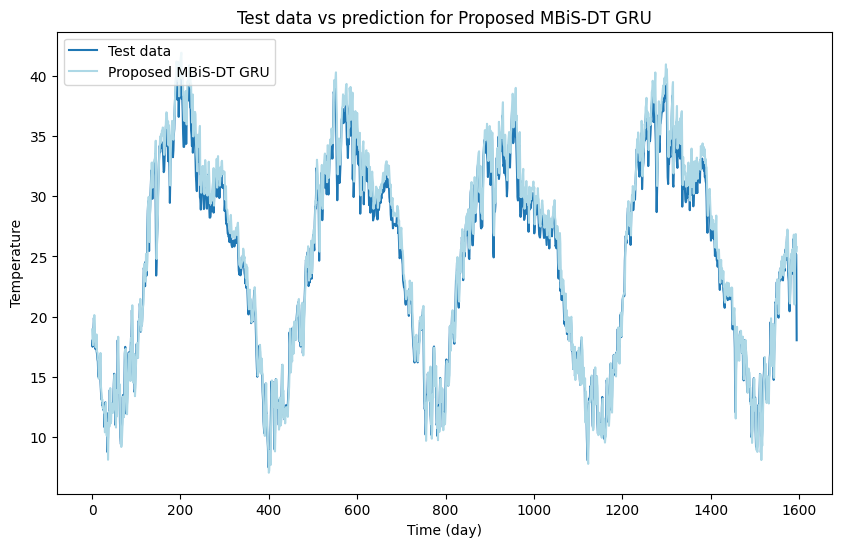
\includegraphics[scale=0.3]{testData_vs_proposed_GRU.png}\label{fig:BarPlot_TestDataVSMBiS-DT_GRU}}
% \hfill
% \subfloat[Test data vs Proposed MBiS-DT RNN]{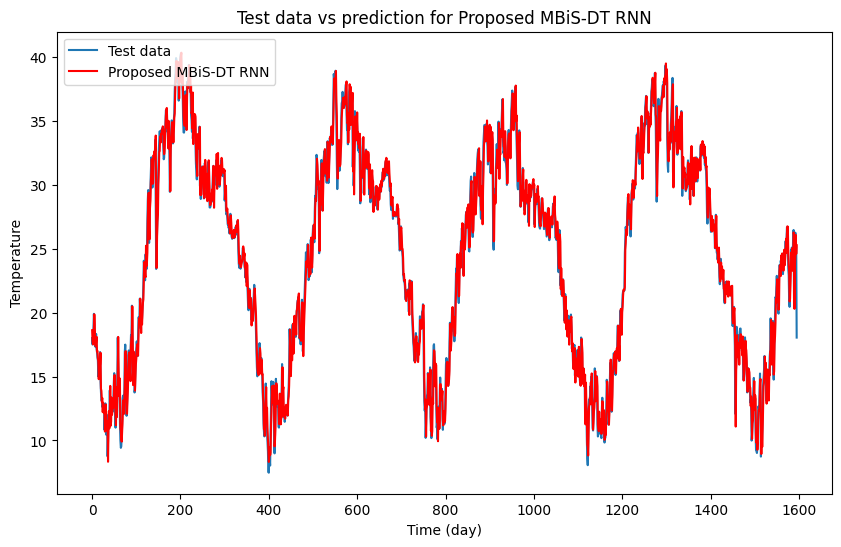
\includegraphics[scale=0.3]{testData_vs_proposed_RNN.png}\label{fig:BarPlot_TestDataVSMBiS-DT_RNN}}\\
% \subfloat[Test data vs Proposed MBiS-DT BI-LSTM]{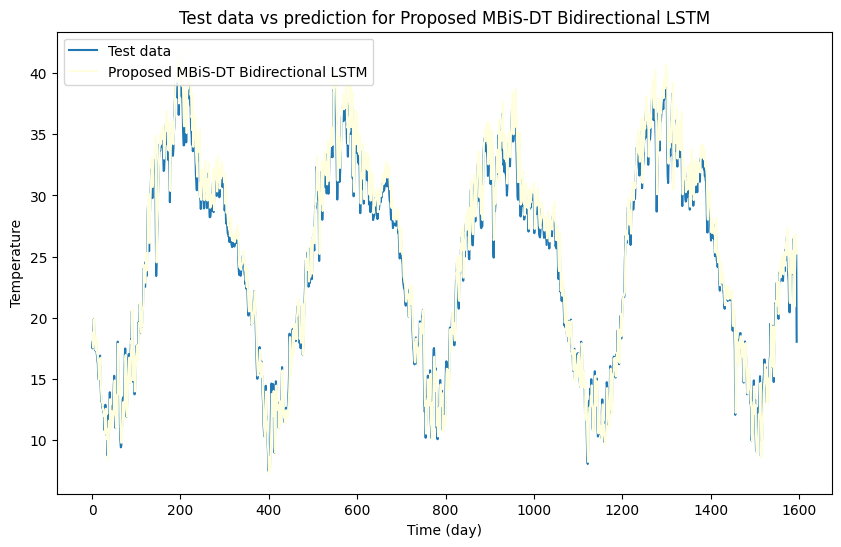
\includegraphics[scale=0.3]{testData_vs_proposed_BI-lstm.png}\label{fig:BarPlot_TestDataVSMBiS-DT_BILSTM}}
% \hfill
% \subfloat[Test data vs Proposed MBiS-DT LSTM]{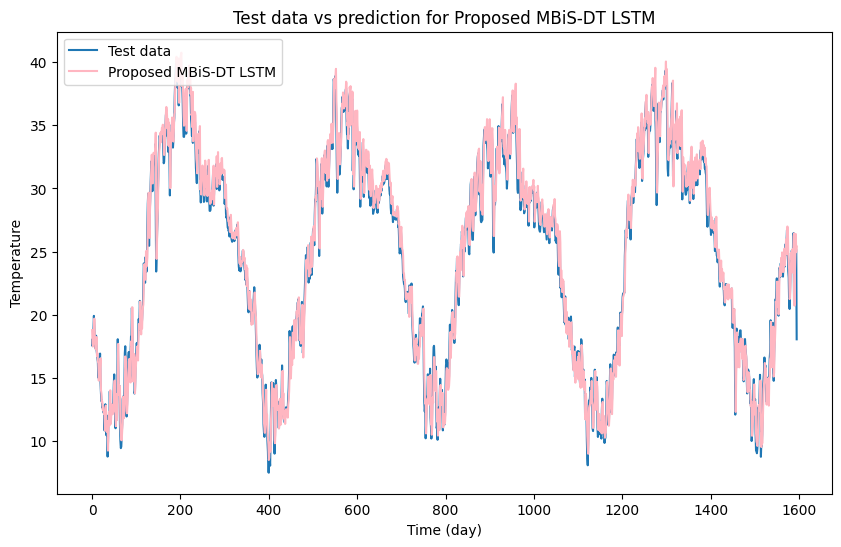
\includegraphics[scale=0.3]{testData_vs_proposed_LSTM.png}\label{fig:BarPlot_TestDataVSMBiS-DT_LSTM}}
% \caption{Prediction plot of original test data(subset) corresponding to traditional DL models and proposed MBiS-DT + DL's models.}
% \label{fig:Line plot of vs proposed MBiS-DT models}
% \end{figure}



% \begin{figure}[ht!]
% \centering
% 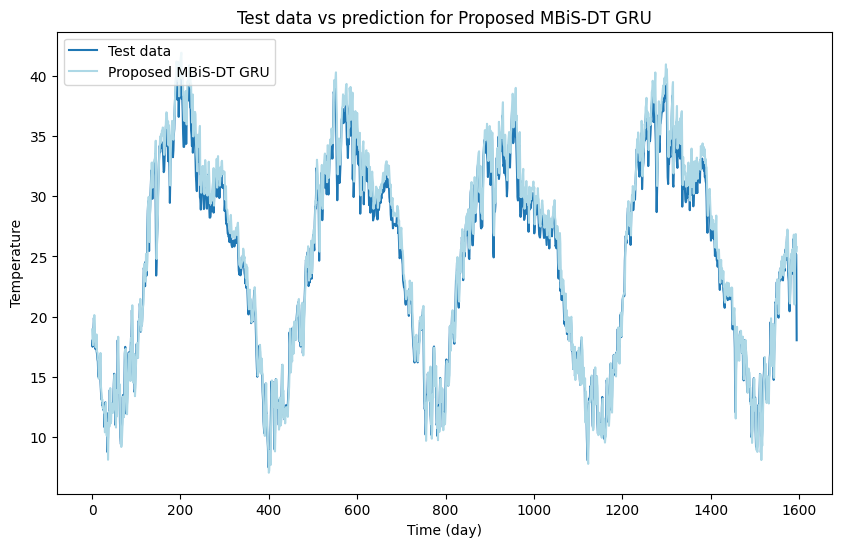
\includegraphics[width=1\textwidth, height=0.9\linewidth]{testData_vs_proposed_GRU.png}
% \caption{Test data vs Proposed MBiS-DT GRU}
% \label{fig:BarPlot_TestDataVSMBiS-DT_GRU}
% \end{figure}
% \begin{figure}[ht!]
% \centering
% 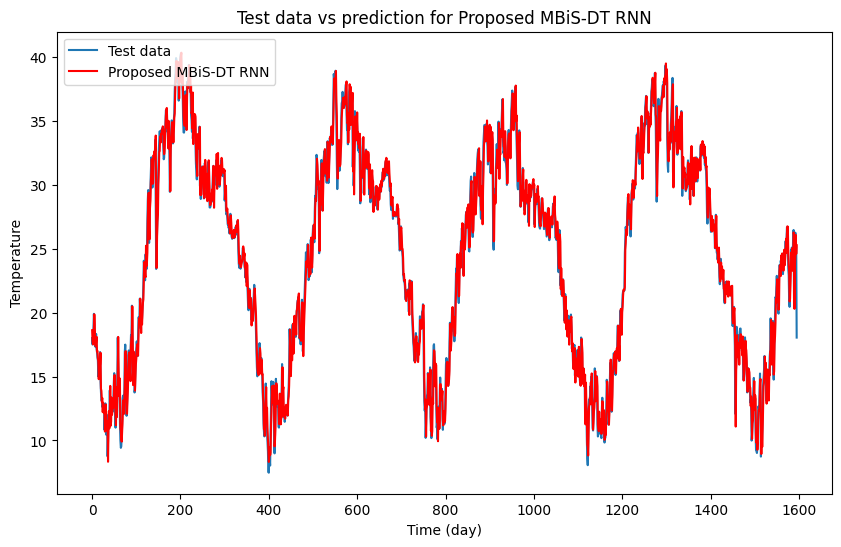
\includegraphics[width=1\textwidth, height=0.9\linewidth]{testData_vs_proposed_RNN.png}
% \caption{Test data vs Proposed MBiS-DT RNN}
% \label{fig:BarPlot_TestDataVSMBiS-DT_RNN}
% \end{figure}
% \begin{figure}[ht!]
% \centering
% 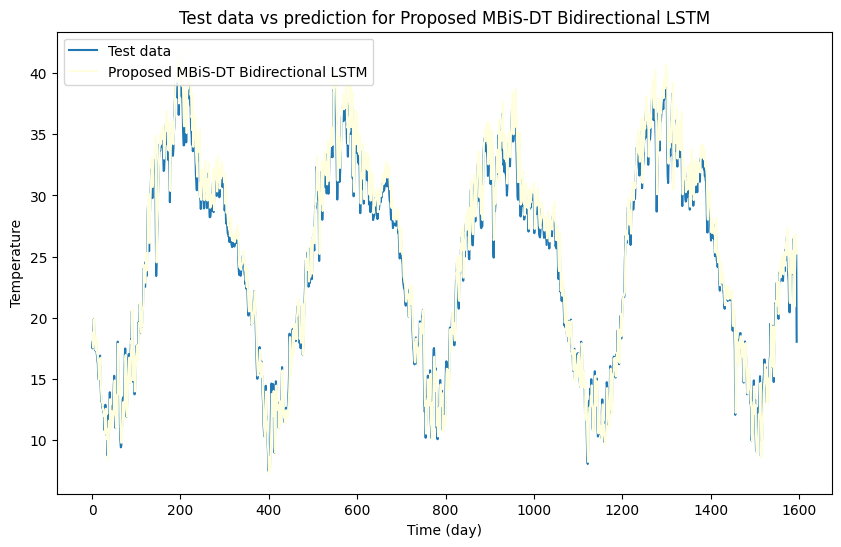
\includegraphics[width=1\textwidth, height=0.9\linewidth]{testData_vs_proposed_BI-lstm.png}
% \caption{Test data vs Proposed MBiS-DT BI-LSTM}
% \label{fig:BarPlot_TestDataVSMBiS-DT_BILSTM}
% \end{figure}
% \begin{figure}[ht!]
% \centering
% 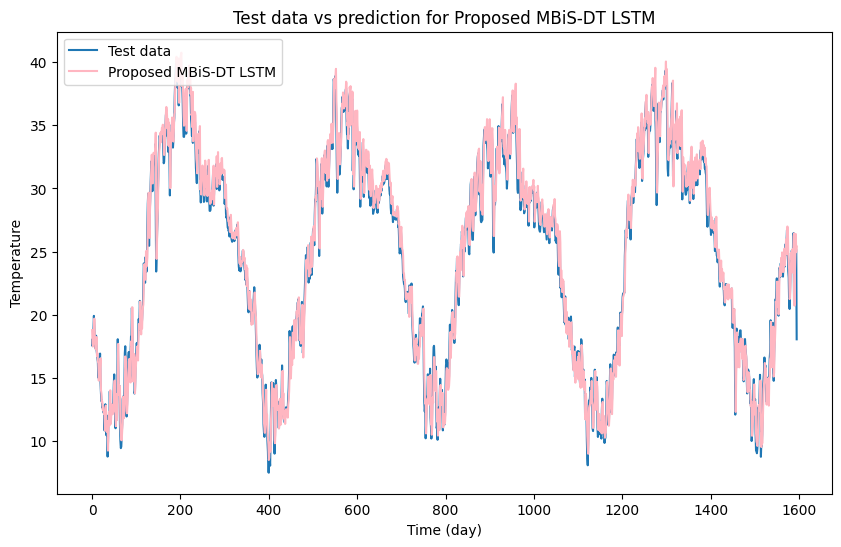
\includegraphics[width=1\textwidth, height=0.9\linewidth]{testData_vs_proposed_LSTM.png}
% \caption{Test data vs Proposed MBiS-DT LSTM}
% \label{fig:BarPlot_TestDataVSMBiS-DT_LSTM}
% \end{figure}



% \begin{figure}[ht!]
% %\centering
% \subfloat[Test data vs Proposed MBiS-DT GRU] {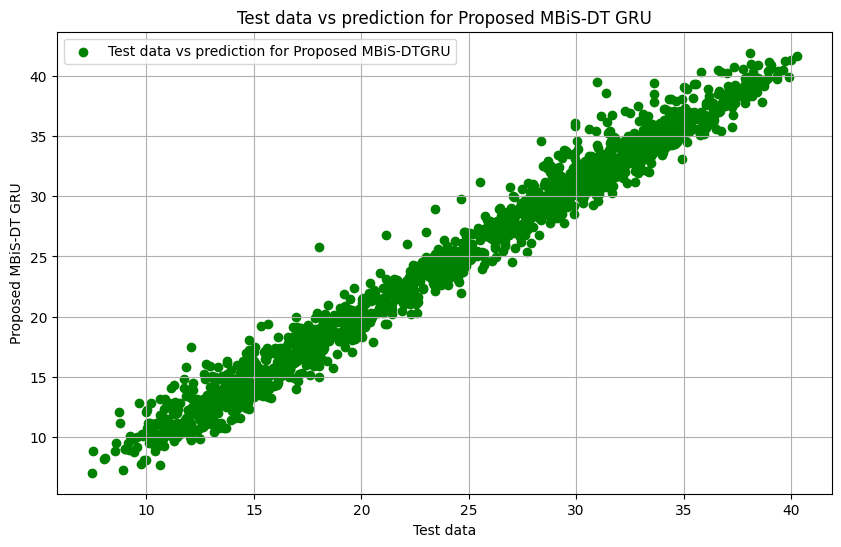
\includegraphics[scale=0.3]{scatter_gru.png}\label{fig:ScatterPlot_TestDataVSMBiS-DT_GRU}}
% \hfill
% \subfloat[Test data vs Proposed MBiS-DT RNN]{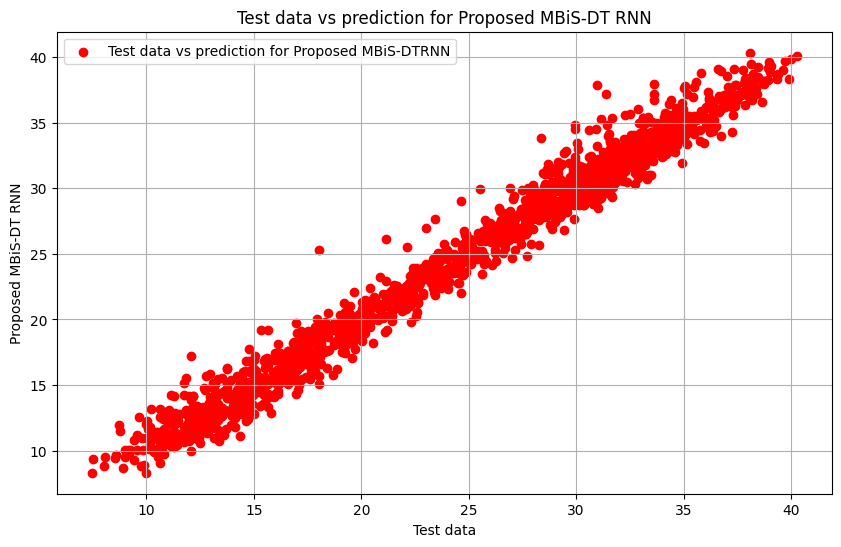
\includegraphics[scale=0.3]{scatter_rnn.png}\label{fig:ScatterPlot_TestDataVSMBiS-DT_RNN}}\\
% \subfloat[Test data vs Proposed MBiS-DT BI-LSTM]{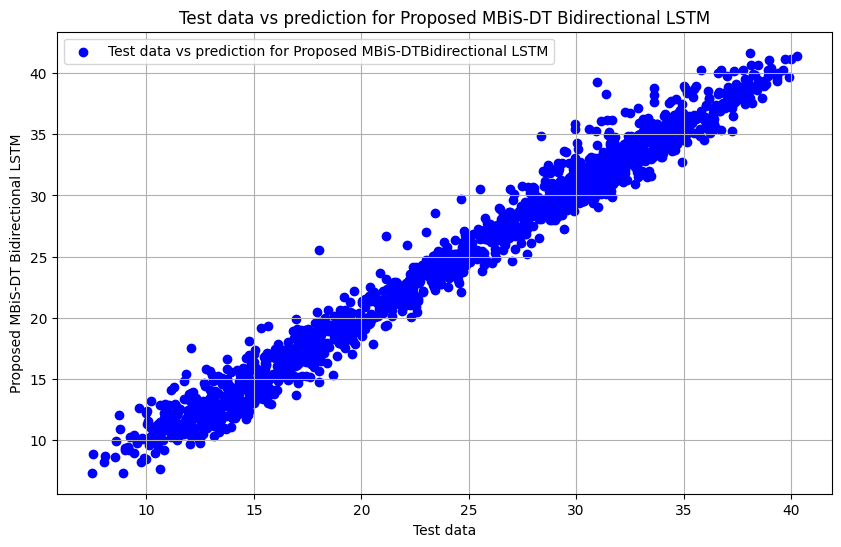
\includegraphics[scale=0.3]{scatter_bilstm.png}\label{fig:ScatterPlot_TestDataVSMBiS-DT_BI-LSTM}}
% \hfill
% \subfloat[Test data vs Proposed MBiS-DT LSTM]{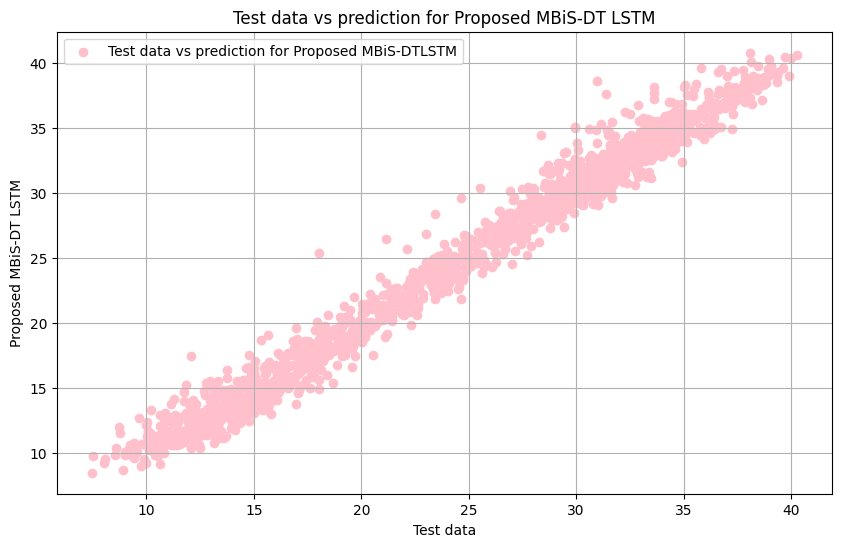
\includegraphics[scale=0.3]{scatter_lstm.png}\label{fig:ScatterPlot_TestDataVSMBiS-DT_LSTM}}
% \caption{Superimposed Prediction Scattered plot of traditional DL and proposed model over test data.}
% \label{fig:Scatter plot of vs proposed MBiS-DT models}
% \end{figure}




% \begin{figure}[ht!]
% \centering
% 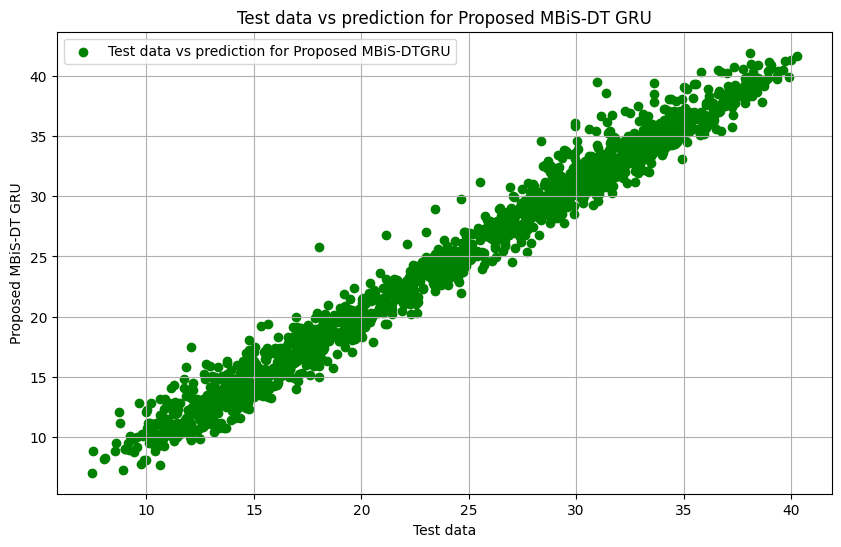
\includegraphics[width=1\textwidth, height=0.9\linewidth]{scatter_gru.png}
% \caption{Test data vs Proposed MBiS-DT GRU}
% \label{fig:ScatterPlot_TestDataVSMBiS-DT_GRU}
% \end{figure}
% \begin{figure}[ht!]
% \centering
% 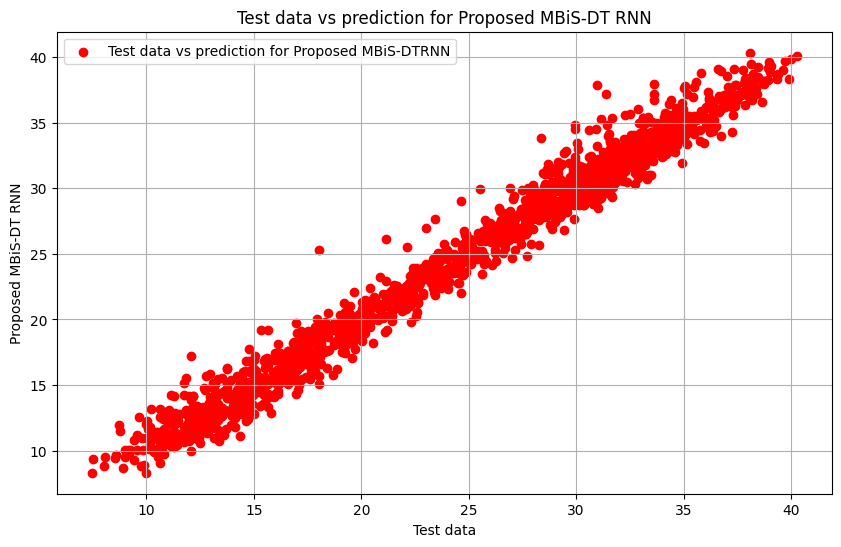
\includegraphics[width=1\textwidth, height=0.9\linewidth]{scatter_rnn.png}
% \caption{Test data vs Proposed MBiS-DT RNN}
% \label{fig:ScatterPlot_TestDataVSMBiS-DT_RNN}
% \end{figure}
% \begin{figure}[ht!]
% \centering
% 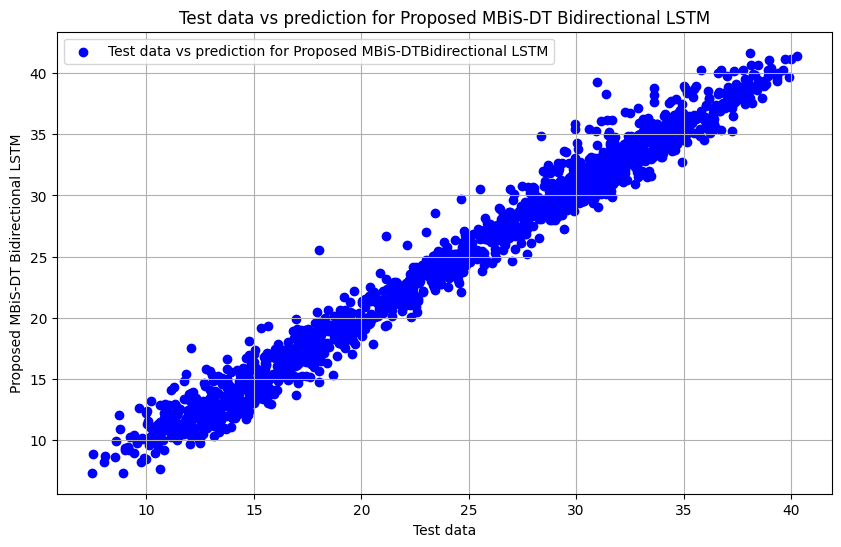
\includegraphics[width=1\textwidth, height=0.9\linewidth]{scatter_bilstm.png}
% \caption{Test data vs Proposed MBiS-DT BI-LSTM}
% \label{fig:ScatterPlot_TestDataVSMBiS-DT_BI-LSTM}
% \end{figure}
% \begin{figure}[ht!]
% \centering
% 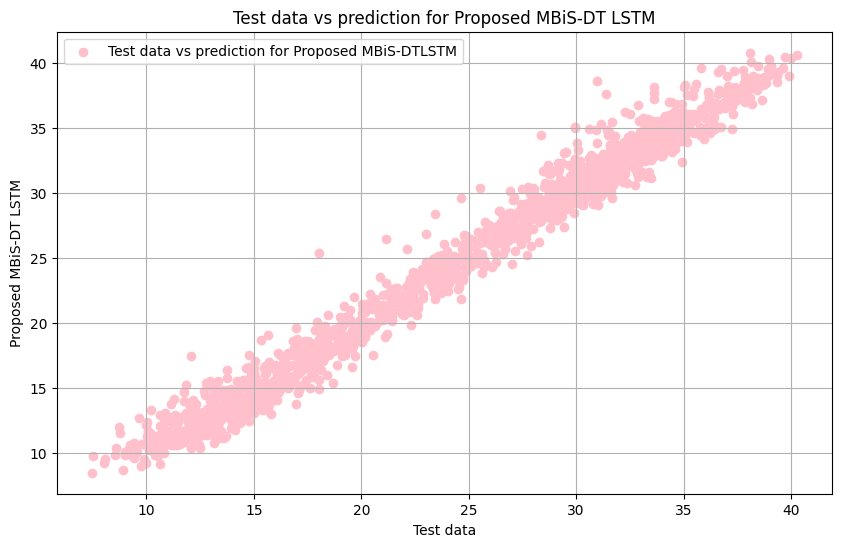
\includegraphics[width=1\textwidth, height=0.9\linewidth]{scatter_lstm.png}
% \caption{Test data vs Proposed MBiS-DT LSTM}
% \label{fig:ScatterPlot_TestDataVSMBiS-DT_LSTM}
% \end{figure}




\section{Performance Measures:}
\subsection{Root Mean Squared Error (RMSE):}
This performance metric is used widely in regression tasks, including temperature prediction. It calculates the average magnitude of the errors between actual and predicted values. The RMSE is calculated by taking the square root of the average of the squared differences between actual and predicted values.

The formula for RMSE is as in eqn. (\ref{eqn:e}):
\begin{equation}
\label{eqn:e}
RMSE = \sqrt {\frac{1}{N} \sum_{i=1}^{N} (\hat{y_{i}} - y_{i})^2}
\end{equation}
where the variables $\hat{y}_i$ is predicted values of the target variable (e.g., temperature), $y_i$ is the actual values of the target variable, and N is the total number of data point in the dataset.
\subsection{Mean Absolute Error (MAE):} It is a data-dependent performance metric used to evaluate the average exact error between actual and predicted variables. The formula for MAE is depicted in eqn. (\ref{eqn:mae})
\begin{equation}
\label{eqn:mae}
MAE = \frac{1}{N} \sum_{i=1}^{N} \left|\hat{y_{i}} - y_{i}\right| .
\end{equation}
where the variables $\hat{y}_i$ are predicted values of the target variable (e.g., temperature), $y_i$ are the actual values of the target variable, and N is the total no. of the data point in the dataset.

\subsection{Mean Squared Error (MSE):}
Mean Squared Error (MSE) is another widely used performance metric in regression tasks, including temperature prediction. It computes the Mean of the squared differences between actual and predicted values. MSE emphasizes a more significant error value than a more minor error value due to the squaring of the differences.
The formula for MSE is as depicted in eqn. (\ref{eqn:mse})
\begin{equation}
\label{eqn:mse}
MSE = \frac{1}{N} \sum_{i=1}^{N} (\hat{y_{i}} - y_{i})^2
\end{equation}
where the variables $\hat{y}_i$ are predicted values of the target variable (e.g., temperature), $y_i$ are the actual values of the target variable, and N is the number of data points in the dataset.


\subsection{Mean Absolute Percentage Error (MAPE):}
Mean Absolute Percentage Error (MAPE) is a performance metric commonly used in regression tasks, including temperature prediction. It measures the average percentage difference between predicted and actual values, providing a relative measure of the accuracy of the model's predictions.

The formula for MAPE is represented in eqn. (\ref{eqn:mape})
\begin{equation}
\label{eqn:mape}
MAPE = \frac{100}{N} \sum_{i=1}^{N} \left|(\frac{\hat{y_{i}} - y_{i}}{y_i})\right| .
\end{equation}

%MAPE = (1/n) * Σ(|(y_actual - y_pred) / y_actual|) * 100

where the variables $\hat{y}_i$ are predicted values of the target variable (e.g., temperature), $y_i$ are the actual values of the target variable, and N is the number of data points in the dataset.



\section{Implementation setup and parameters settings}
The various packages of Python are utilized to implement the baseline and proposed models. These include Pandas (v1.5.3), Scikit-Learn (v1.2.2) for model creation and performance analysis, Keras (v2.12.0), TensorFlow (v2.12.0) for Keras backend, and NumPy (v1.23.5) for exploratory data analysis, and For describing the findings and creating graphs, we used Plotly (v5.14.1), seaborn (v0.12.2), and Matplotlib (v3.7.1). To create flowcharts, it has also used \href{https://docs.google.com/drawings/}{https://docs.google.com/drawings/}. One system was employed for the experiments: a MacOS-based computer with Apple M1 having 8 GB RAM. All experiments were done on Google Colab with runtime Python 3 and hardware-accelerated T4 GPU with 12.7 GB RAM. Table \ref{tab: my-table} has the parameter values of the traditional DL and proposed models.

\begin{table*}[h!]
\centering
\setlength{\tabcolsep}{3pt}
{\renewcommand{\arraystretch}{1}%

\caption{Parameter setting of traditional DL models and proposed MBiS-DT Models}
\label{tab: my-table}
\begin{tabular}{ll}
\hline Hyperparameters & Values \\ \hline
Batch Size & 32 \\
Optimizer & Adam \\
Loss function & Mean Squared Error \\
Epoch & 200 with early stopping \\
training size & 0.8 \\ \hline
\end{tabular}}
\end{table*}
Upward batch and Downward batch ensemble(UD-Batch) and Corresponding upward and downward ensemble(CUD-ensemble)

